\documentclass{article}

\usepackage{fancyhdr}
\usepackage{extramarks}
\usepackage{amsmath}
\usepackage{amsthm}
\usepackage{amssymb}
\usepackage{amsfonts}
\usepackage{tikz}
\usepackage[plain]{algorithm}
\usepackage{algpseudocode}
\usepackage{float} 
\usepackage{cancel}
\usepackage{algorithm}


\usetikzlibrary{automata,positioning}

%
% Basic Document Settings
%

\topmargin=-0.45in
\evensidemargin=0in
\oddsidemargin=0in
\textwidth=6.5in
\textheight=9.0in
\headsep=0.25in

\linespread{1.1}

\pagestyle{fancy}
\lhead{\hmwkAuthorName}
\chead{\hmwkClass\ \hmwkTitle}
%\chead{\hmwkClass\ (\hmwkClassInstructor\ \hmwkClassTime): \hmwkTitle}
\rhead{\firstxmark}
\lfoot{\lastxmark}
\cfoot{\thepage}

\renewcommand\headrulewidth{0.4pt}
\renewcommand\footrulewidth{0.4pt}

\setlength\parindent{0pt}

%
% Create Problem Sections
%

\newcommand{\enterProblemHeader}[1]{
    \nobreak\extramarks{}{Problem \arabic{#1} continued on next page\ldots}\nobreak{}
    \nobreak\extramarks{Problem \arabic{#1} (continued)}{Problem \arabic{#1} continued on next page\ldots}\nobreak{}
}

\newcommand{\exitProblemHeader}[1]{
    \nobreak\extramarks{Problem \arabic{#1} (continued)}{Problem \arabic{#1} continued on next page\ldots}\nobreak{}
    \stepcounter{#1}
    \nobreak\extramarks{Problem \arabic{#1}}{}\nobreak{}
}

\setcounter{secnumdepth}{0}
\newcounter{partCounter}
\newcounter{homeworkProblemCounter}
\setcounter{homeworkProblemCounter}{1}
\nobreak\extramarks{Problem \arabic{homeworkProblemCounter}}{}\nobreak{}

%
% Homework Problem Environment
%
% This environment takes an optional argument. When given, it will adjust the
% problem counter. This is useful for when the problems given for your
% assignment aren't sequential. See the last 3 problems of this template for an
% example.
%
\newenvironment{homeworkProblem}[1][-1]{
    \ifnum#1>0
        \setcounter{homeworkProblemCounter}{#1}
    \fi
    \section{Problem \arabic{homeworkProblemCounter}}
    \setcounter{partCounter}{1}
    \enterProblemHeader{homeworkProblemCounter}
}{
    \exitProblemHeader{homeworkProblemCounter}
}

%
% Homework Details
%   - Title
%   - Due date
%   - Class
%   - Section/Time
%   - Instructor
%   - Author
%

\newcommand{\hmwkTitle}{Homework\ \#4}
\newcommand{\hmwkDueDate}{March 17, 2022 (2 days free late.)}
\newcommand{\hmwkClass}{EECS 545 Machine Learning}
\newcommand{\hmwkClassTime}{Section A}
\newcommand{\hmwkClassInstructor}{Professor Honglak Lee}
\newcommand{\hmwkAuthorName}{\textbf{Yuang Huang}}
\newcommand{\hmwkUninameName}{\textbf{yahuang@umich.edu}}

%
% Title Page
%

\title{
    \vspace{2in}
    \textmd{\textbf{\hmwkClass:\ \hmwkTitle}}\\
    \normalsize\vspace{0.1in}\small{Due\ on\ \hmwkDueDate\ at 11:59pm}\\
    \vspace{0.1in}\large{\textit{\hmwkClassInstructor\ \hmwkClassTime}}
    \vspace{3in}
}

\author{\hmwkAuthorName\\
\hmwkUninameName}
\date{}

\renewcommand{\part}[1]{\textbf{\large Part \Alph{partCounter}}\stepcounter{partCounter}\\}

%
% Various Helper Commands
%

% Useful for algorithms
\newcommand{\alg}[1]{\textsc{\bfseries \footnotesize #1}}

% For derivatives
\newcommand{\deriv}[1]{\frac{\mathrm{d}}{\mathrm{d}x} (#1)}

% For partial derivatives
\newcommand{\pderiv}[2]{\frac{\partial}{\partial #1} (#2)}

% Integral dx
\newcommand{\dx}{\mathrm{d}x}

% Alias for the Solution section header
\newcommand{\solution}{\textbf{\large Solution}}

% Probability commands: Expectation, Variance, Covariance, Bias
\newcommand{\E}{\mathrm{E}}
\newcommand{\Var}{\mathrm{Var}}
\newcommand{\Cov}{\mathrm{Cov}}
\newcommand{\Bias}{\mathrm{Bias}}

\begin{document}

\maketitle

\pagebreak

\begin{homeworkProblem}
    \large {Neural Network Layer Implementation}
    \\
    \textbf{Solution}

    \begin{equation}
    \mathbf{w}_{\rm ML} = \underset{\mathbf{w}}{\mathrm{argmax}} \prod_{i=1}^{N}p(y^{(i)}|\mathbf{x^{(i)}; \mathbf{w}}),
    \label{eq1}
    \end{equation}

    \begin{equation}
        \mathbf{w}_{\rm MAP} = \underset{\mathbf{w}}{\mathrm{argmax}} \, p(\mathbf{w})\prod_{i=1}^{N}p(y^{(i)}|\mathbf{x^{(i)}; \mathbf{w}}).
    \label{eq2}
    \end{equation}
    So we will have:
    \begin{equation}
        \mathbf{w}_{\rm ML} = \underset{\mathbf{w}}{\mathrm{argmin}} \,  - (\sum_{i=1}^{N}\log p(y^{(i)}|\mathbf{x^{(i)}; \mathbf{w}})),
    \label{eq3}
    \end{equation}

    \begin{equation}
        \mathbf{w}_{\rm MAP} = \underset{\mathbf{w}}{\mathrm{argmin}} \,  - (\log p(\mathbf{w}) + \sum_{i=1}^{N}\log p(y^{(i)}|\mathbf{x^{(i)}; \mathbf{w}})).
    \label{eq4}
    \end{equation}
    Because the prior $\mathbf{w} \sim \mathcal{N}(0, \tau^2 I)$, the value of $p(\mathbf{w})$ will decrease 
    monotonically with $||\mathbf{w}||$, and then we will know $\log(\mathbf{w}) \propto ||\mathbf{w}||_2$ for MAP.
    We assume that $||\mathbf{w_{MAP}}||_2 > ||\mathbf{w_{ML}}||_2$, then we get:
    \begin{equation}
    \begin{aligned}
     &- (\log p(\mathbf{w_{MAP}}) + \sum_{i=1}^{N}\log p(y^{(i)}|\mathbf{x^{(i)}; \mathbf{w_{MAP}}})) - (- (\log p(\mathbf{w_{ML}}) + \sum_{i=1}^{N}\log p(y^{(i)}|\mathbf{x^{(i)}; \mathbf{w_{ML}}})) )\\
     &= \log{\frac{p(\mathbf{w}_{ML})}{p(\mathbf{w}_{MAP})}} - \sum_{i=1}^{N}\log p(y^{(i)}|\mathbf{x^{(i)}; \mathbf{w_{ML}}}) + \sum_{i=1}^{N}\log p(y^{(i)}|\mathbf{x^{(i)}; \mathbf{w_{MAP}}})
    \label{eq5}
    \end{aligned}
    \end{equation}
    From ($\ref{eq1}$) we know that $\sum_{i=1}^{N}\log p(y^{(i)}|\mathbf{x^{(i)}; \mathbf{w_{MAP}}}) < \sum_{i=1}^{N}\log p(y^{(i)}|\mathbf{x^{(i)}; \mathbf{w_{ML}}})$, so the above equation is smaller than 
    zero which contradicts to ($\ref{eq4}$) because $\mathbf{w}_{\rm ML}$ for the term $'' \underset{\mathbf{w}}{\mathrm{argmin}} \,  - (\log p(\mathbf{w}) + \sum_{i=1}^{N}\log p(y^{(i)}|\mathbf{x^{(i)}; \mathbf{w}})) ''$ has 
    smaller value than $\mathbf{w}_{\rm MAP}$. So our assumption is wrong, it can be proved that:
    \begin{equation}
        ||\mathbf{w}_{\rm MAP}|| \leq ||\mathbf{w}_{\rm ML}||
        \label{eq16}
    \end{equation}

\end{homeworkProblem}

\pagebreak

\begin{homeworkProblem}
    \large Direct construction of valid kernels\\

    \textbf{Solution}

    \textbf{Part a:}\\
    $\bullet$ Symmetric

    Because $k_1(\mathbf{x}, \mathbf{z})$ and $k_2(\mathbf{x}, \mathbf{z})$ are kernels,  $k_1(\mathbf{x}, \mathbf{z}) = k_1(\mathbf{z}, \mathbf{x})$
    and  $k_2(\mathbf{x}, \mathbf{z}) = k_2(\mathbf{z}, \mathbf{x})$. Then it is obviously that  $k(\mathbf{x}, \mathbf{z}) = k(\mathbf{z}, \mathbf{x})$
    so the matrix $K$ is symmetric.

    $\bullet$ positive semi-definite

    Because $k_1(\mathbf{x}, \mathbf{z})$ and $k_2(\mathbf{x}, \mathbf{z})$ are kernels,
    $x^TK_1x \geq 0$ and $y^TK_2y \geq 0$. It is obviously that $x^TKx = x^TK_1x + x^TK_2x \geq 0$, so the 
    matrix $K$ is positive semi-definite. \\


    \textbf{Part b:}\\
    It is not a kernal.

    Counterexample: We assume that :
    \begin{gather}
        K_1 = 
        \begin{pmatrix} 
            1 & 0 \\ 0 & 1 
        \end{pmatrix}
        K_2 = 
        \begin{pmatrix} 
            3 & 0 \\ 0 & 3 
        \end{pmatrix}
    \end{gather}
    
    Because both $K_1$ and $K_2$ are symmetric and positive semi-definite, both $k_1$ and $k_2$
    are kernels. So the matrix $K$:
    \begin{gather}
        K = K_1 - K_2 = 
        \begin{pmatrix} 
            -2 & 0 \\ 0 & -2 
        \end{pmatrix},
    \end{gather}
    we choose a vector $x = [1 \quad 1]^T$, then we will get
    \begin{gather}
        x^TKx = 
        \begin{pmatrix} 
            -4 
        \end{pmatrix} < 0.
    \end{gather}
    Thus, it is not a kernel.\\
    
    \textbf{Part c:}\\
    $\bullet$ Symmetric

    Because $k_1(\mathbf{x}, \mathbf{z})$ is a kernel, $k_1(\mathbf{x}, \mathbf{z}) = k_1(\mathbf{z}, \mathbf{x})$. Thus, $ak_1(\mathbf{x}, \mathbf{z}) = ak_1(\mathbf{z}, \mathbf{x})$.
    So the matrix $K$ is symmetric.

    $\bullet$ positive semi-definite

    Because $k_1(\mathbf{x}, \mathbf{z})$ is a kernel,
    $x^TK_1x \geq 0$. It is obviously that $x^TKx = ax^TK_1x \geq 0$ where a is $a$ positive real number, so the 
    matrix $K$ is positive semi-definite.\\





    \textbf{Part d:}\\
    It is not a kernal.

    Counterexample: We assume that : $a = 1$
    \begin{gather}
        K_1 = 
        \begin{pmatrix} 
            1 & 0 \\ 0 & 1 
        \end{pmatrix}
        K = 
        \begin{pmatrix} 
            -1 & 0 \\ 0 & -1 
        \end{pmatrix}
    \end{gather}
    
    we choose a vector $x = [1 \quad 1]^T$, then we will get
    \begin{gather}
        x^TKx = 
        \begin{pmatrix} 
            -2 
        \end{pmatrix} < 0.
    \end{gather}
    Thus, it is not a kernel.

    \textbf{Part e:}\\
    $\bullet$ Symmetric

    Because $k_1(\mathbf{x}, \mathbf{z})$ and $k_2(\mathbf{x}, \mathbf{z})$ are kernels,  $k_1(\mathbf{x}, \mathbf{z}) = k_1(\mathbf{z}, \mathbf{x})$
    and  $k_2(\mathbf{x}, \mathbf{z}) = k_2(\mathbf{z}, \mathbf{x})$. Then it is obviously that  $k(\mathbf{x}, \mathbf{z}) = k_1(\mathbf{x}, \mathbf{z})k_2(\mathbf{x}, \mathbf{z})
     = k_1(\mathbf{z}, \mathbf{x})k_2(\mathbf{z}, \mathbf{x}) = k(\mathbf{z}, \mathbf{x})$,
    so the matrix $K$ is symmetric.

    $\bullet$ positive semi-definite

    Because $k_1(\mathbf{x}, \mathbf{z})$ and $k_2(\mathbf{x}, \mathbf{z})$ are kernels,
    $x^TK_1x \geq 0$ and $y^TK_2y \geq 0$. $K_{(1)ij} = \sum_k^Du_{ik} \lambda_k u_{kj}$ where 
    $K_1 = \mathbf{U}^T \Lambda \mathbf{U}$. Thus, 
    \begin{equation}
        \begin{aligned}
            x^TKx &= \sum_i^D\sum_j^Dx_iK_{(1)ij}K_{(2)ij}x_j\\
            &= \sum_i^D\sum_j^D\sum_k^Dx_iu_{ij} \lambda_k u_{kj}K_{(2)ij}x_j\\
            &= \sum_i^D\sum_j^D\sum_k^D \lambda_kx_iu_{ik}K_{(2)ij}u_{kj}x_j\\
        \end{aligned}
    \end{equation}
    We know $\lambda \geq 0$ because 
     $K_1$ is positive semi-definite. Thus, $\sum_i^D\sum_j^D\sum_k^D \lambda_kx_iu_{ik}K_{(2)ij}u_{kj}x_j = 
     \sum_i^D\sum_j^D\sum_k^D \lambda_kt_{ik}K_{(2)ij}t_{kj} \geq 0$ because $K_2$ is positive semi-definite.
    So, the matrix $K$ is positive semi-definite.

    \textbf{Part f:}\\
    $\bullet$ Symmetric

    We can get $k(\mathbf{x}, \mathbf{z}) = f(\mathbf{x})f(\mathbf{z}) = f(\mathbf{z})f(\mathbf{x}) = k(\mathbf{z}, \mathbf{x})$. 
    Thus, the matrix $K$ is symmetric.

    $\bullet$ positive semi-definite

    Because $K_{ij} = f(\mathbf{x}_i)f(\mathbf{x}_j)$, then we will get:
    \begin{equation}
    \begin{aligned}
        \mathbf{y}^TK\mathbf{y} &= \sum_i^D\sum_j^Dy_iK_{ij}y_j\\
        & = \sum_i^D\sum_j^Dy_if(\mathbf{x}_i)f(\mathbf{x}_j)y_j\\
        & = \sum_i^D[y_if(\mathbf{x_i})]^2 + \sum_{i \neq j}^D2y_if(\mathbf{x}_i)f(\mathbf{x}_j)y_j\\
        & = \sum_i^D [y_if(\mathbf{x}_i) + y_jf(\mathbf{x}_j)]^2 \geq 0.
    \end{aligned}
    \end{equation}
    Thus, the matrix $K$ is positive semi-definite.
    \\
    \textbf{Part g:}\\
    $\bullet$ Symmetric

    Because $k_3$ is a kernel, $k(\mathbf{x}, \mathbf{z}) = k_3(\phi(\mathbf{x}), 
    \phi(\mathbf{z})) = k_3(\phi(\mathbf{z}), \phi(\mathbf{x}))
     = k(\mathbf{z}, \mathbf{x})$. 
    So the matrix $K$ is symmetric.

    $\bullet$ positive semi-definite

    Because $k_3$ is a kernel, $x^TK_3x \geq 0$. 
    \begin{equation}
        \begin{aligned}
            \mathbf{y}^TK\mathbf{y} &= \sum_i^D\sum_j^Dy_iK_{ij}y_j\\
            & = \sum_i^D\sum_j^Dy_ik(\mathbf{x}^{(i)}, \mathbf{x}^{(j)})y_j\\
            & = \sum_i^D\sum_j^Dy_ik_3(\phi(\mathbf{x}^{(i)}), \phi(\mathbf{x}^{(j)}))y_j \geq 0.
        \end{aligned}
    \end{equation}
    Thus, the matrix $K$ is positive semi-definite.\\

    \textbf{Part h:}\\
    $\bullet$ Symmetric

    Because $k_1$ is a kernel, $k_1(\mathbf{x}, \mathbf{z}) = k_1(\mathbf{z}, \mathbf{x}) 
    \Rightarrow [k_1(\mathbf{x}, \mathbf{z})]^n = [k_1(\mathbf{z}, \mathbf{x})]^n
    \Rightarrow a_n[k_1(\mathbf{x}, \mathbf{z})]^n = a_n[k_1(\mathbf{z}, \mathbf{x})]^n
    \Rightarrow k(\mathbf{x}, \mathbf{z}) = \sum_1^N a_n[k_1(\mathbf{x}, \mathbf{z})]^n
    = \sum_1^N a_n[k_1(\mathbf{z}, \mathbf{x})]^n = k(\mathbf{z}, \mathbf{x}).
    $
    So the matrix $K$ is symmetric.

    $\bullet$ positive semi-definite

    From (e), we know $k(\mathbf{x}, \mathbf{z}) 
    = k_1(\mathbf{x}, \mathbf{z})k_2(\mathbf{x}, \mathbf{z})$ is a kernel. Let 
    $k_2(\mathbf{x}, \mathbf{z}) = k_1(\mathbf{x}, \mathbf{z})$, then we will get
    $k_1(\mathbf{x}, \mathbf{z})k_1(\mathbf{x}, \mathbf{z}) = [k_1(\mathbf{x}, \mathbf{z})]^2$
    is a kernel. Also, we can get that $k_1(\mathbf{x}, \mathbf{z})[k_1(\mathbf{x}, \mathbf{z})]^2 = [k_1(\mathbf{x}, \mathbf{z})]^3$
    is a kernel. Thus, we will know that $[k_1(\mathbf{x}, \mathbf{z})]^n$ is always a kernel 
    where n is an positive integer number. In addition, we have $\mathbf{y}^Ta_n[k_1(\mathbf{x}, \mathbf{z})]^n\mathbf{y} \geq 0$ where
    $a_n$ is a positive coefficeint. So, $\mathbf{y}^TK\mathbf{y} = \mathbf{y}^T\sum_1^N a_n[k_1(\mathbf{x}, \mathbf{z})]^n\mathbf{y}
    = \sum_1^N \mathbf{y}^Ta_n[k_1(\mathbf{x}, \mathbf{z})]^n\mathbf{y} \geq 0.$ 
    Thus, the matrix $K$ is positive semi-definite.
    
    \textbf{Part i:}\\
    $k(\mathbf{x}, \mathbf{z}) = (\mathbf{x}^T\mathbf{z} + 1)^2$. We assume $\mathbf{D} = 2$, then 
    $\mathbf{x} = [x_1 \quad x_2]^T$, $\mathbf{z} = [z_1 \quad z_2]^T$. Thus, $k(\mathbf{x}, \mathbf{z}) 
    = (x_1z_1+ x_2z_2 + 1)^2 = x_1^2z_1^2 + x_2^2z_2^2 + 2x_1z_1 + 2x_2z_2 + 2x_1x_2z_1z_2 + 1
    = \phi(\mathbf{x})^T\phi(\mathbf{z})$, so $\phi(\mathbf{x}) = (x_1^2, x_2^2, \sqrt{2}x_1, \sqrt{2}x_2, \sqrt{2}x_1x_2, 1).$

    \pagebreak

    \textbf{Part j:}\\
    \begin{equation}
        \begin{aligned}
            k(\mathbf{x}, \mathbf{z}) &= \exp(\frac{-||\mathbf{x} - \mathbf{z}||^2}{2\sigma^2}) \\
            & = \exp(\frac{-\mathbf{x}^T\mathbf{x} - \mathbf{z}^T\mathbf{z} + 2\mathbf{x}^T\mathbf{z}}{2\sigma^2})\\
            & = \exp(\frac{-\mathbf{x}^T\mathbf{x}}{{2\sigma^2}})\times\exp(\frac{-\mathbf{z}^T\mathbf{z}}{{2\sigma^2}})\times\exp(\frac{\mathbf{x}^T\mathbf{z}}{{\sigma^2}}).
        \end{aligned}
    \end{equation}

    Also, we know $\mathbf{x}^T\mathbf{z} = \sum_{k=1}^{\infty} x_kz_k$, so the third term $\exp(\frac{\mathbf{x}^T\mathbf{z}}{{\sigma^2}})$
    can be expressed by:
    \begin{equation}
        \begin{aligned}
            &\exp(\frac{\mathbf{x}^T\mathbf{z}}{{\sigma^2}}) = \exp(\frac{ \sum_{k=1}^{\infty} x_kz_k}{\sigma^2}) \\
            & = \sum_{k=1}^{\infty}\sum_{n = 0}^{\infty}\frac{ (\frac{\sum_{k=1}^{\infty} x_kz_k}{\sigma^2})^n}{n!}\\
            & = \sum_{n=0}^{\infty}\sum_{\sum_{t_D} = n}\frac{C_n^{t_1}C_{n - t_1}^{t_2}C_{n - t_1 - t_2}^{t_3}\cdots C_{t_D}^{t_D}(\frac{x_1z_1}{\sigma^2})^{t_1}
            (\frac{x_2z_2}{\sigma^2})^{t_2}\cdots (\frac{x_Dz_D}{\sigma^2})^{t_D}}{n!}\\
            & = \sum_{n=0}^{\infty}\sum_{\sum_{t_D} = n}\frac{\frac{n!}{t_1!(n-t_1)!}\frac{(n - t_1)!}{t_2!(n-t_1-t_2)!}\cdots \frac{(n - t_1 - \cdots t_{D - 2})!}{t_{D-1}!(n-t_1-\cdots t_{D-1})!}(\frac{x_1z_1}{\sigma^2})^{t_1}
            (\frac{x_2z_2}{\sigma^2})^{t_2}\cdots (\frac{x_Dz_D}{\sigma^2})^{t_D}}{n!}\\
            & = \sum_{n=0}^{\infty}\sum_{\sum_{t_D} = n}\frac{1}{t_1!\cancel{(n-t_1)!}}\frac{\cancel{(n - t_1)!}}{t_2!\cancel{(n-t_1-t_2)!}}\cdots \frac{\cancel{(n - t_1 - \cdots t_{D - 2})!}}{t_{D-1}!t_D!}(\frac{x_1z_1}{\sigma^2})^{t_1}
            (\frac{x_2z_2}{\sigma^2})^{t_2}\cdots (\frac{x_Dz_D}{\sigma^2})^{t_D}\\
            & = \sum_{n=0}^{\infty}\sum_{\sum_{t_D} = n}\frac{1}{t_1!}\frac{1}{t_2!}\cdots \frac{1}{t_D!}(\frac{x_1z_1}{\sigma^2})^{t_1}
            (\frac{x_2z_2}{\sigma^2})^{t_2}\cdots (\frac{x_Dz_D}{\sigma^2})^{t_D}\\
            & = \sum_{n=0}^{\infty}\sum_{\sum_{t_D} = n}\frac{(\frac{{x_1}}{\sigma})^{t_1}{(\frac{{x_2}}{\sigma})}^{t_2}\cdots {(\frac{{x_D}}{\sigma})}^{t_D}}{\sqrt{t_1!}\sqrt{t_2!}\cdots \sqrt{t_D!}}
            \frac{{(\frac{{z_1}}{\sigma})}^{t_1}{(\frac{{z_2}}{\sigma})}^{t_2}\cdots {(\frac{{z_D}}{\sigma})}^{t_D}}{\sqrt{t_1!}\sqrt{t_2!}\cdots \sqrt{t_D!}}
        \end{aligned}
    \end{equation}

    Thus, the closed form of an infinite dimensional feature vector $\phi$ can be written by:
    \begin{equation}
        \phi(\mathbf{x}) = (\exp(\frac{-\mathbf{x}^T\mathbf{x}}{2\sigma^2}),
        \frac{{x_1}^{t_1}{x_2}^{t_2}\cdots {x_D}^{t_D}}{\sqrt{t_1!}\sqrt{t_2!}\cdots \sqrt{t_D!}\sigma^n} for\, all\, possible\, terms, \cdots)
    \end{equation}
\end{homeworkProblem}

\pagebreak

\begin{homeworkProblem}
    \large Kernelizing the Perceptron\\

    \textbf{Solution}

    \textbf{Part a(\romannumeral1):}\\
    $\bullet$ If $y^{(n)}h > 0$, then $\mathbf{w}_{t+1} = \mathbf{w}_t = \Phi^T\mathbf{\alpha}_t$, and we have $\mathbf{\alpha}_{t+1} = \mathbf{\alpha}_t$\\
    $\bullet$ If $y^{(n)}h < 0$, then $\mathbf{w}_{t+1} = \mathbf{w}_t + y^{(n)}\mathbf{x}^{(n)} 
    = \Phi^T\mathbf{\alpha}_t + y^{(n)}\phi(\mathbf{x}^{(n)}) = \Phi^T\mathbf{\alpha}_t + \Phi^T\mathbf{\alpha}_{+},$
    where 
    \begin{equation}
        \mathbf{\alpha}_{+i}=\left\{
        \begin{array}{ll} 
        y^{(n)}, &i = n \\
        0, &i \neq n 
        \end{array}
        \right.
        \label{eqa1}
    \end{equation}
    Thus, $\mathbf{w}_{t+1} =  \Phi^T(\mathbf{\alpha}_{+} + \mathbf{\alpha}_{t}) = \Phi^T\mathbf{\alpha}_{t+1}$,
    where $\mathbf{\alpha}_{t+1} = \mathbf{\alpha}_{t} + \mathbf{\alpha}_{+}$
    \\
    

    \textbf{Part a(\romannumeral2):}\\
    Assume $\mathbf{w}_0 = 0 = \Phi^T\times0$,\\
    then we will have $\mathbf{w}_1 = 0 + \Phi^T\mathbf{\alpha_{+}}= \Phi^T\times\mathbf{\alpha}_1$,\\
    then we will have $\mathbf{w}_2 = \mathbf{w_1} + \Phi^T\mathbf{\alpha_{+}}= \Phi^T\times\mathbf{\alpha_{1}} + \Phi^T\times\mathbf{\alpha_{+}} = \Phi^T\times\mathbf{\alpha}_2$,\\
    $\cdots$\\
    $\mathbf{w}_t = \Phi^T\times \alpha_t$ and $\mathbf{w}_{t+1} = \Phi^T\times (\alpha_t + \alpha_+) = \Phi^T\times \alpha_{t+1}$ from a(\romannumeral1).\\
    Thus, for $0 \leq t \leq T$, $\mathbf{w}_t$ can be expressed as $\Phi^T\alpha_t$.\\

    \textbf{Part b(\romannumeral1):}\\
    $\bullet$ If $y^{(n)}h > 0$, then $\mathbf{w}_{t+1} = \mathbf{w}_t = \Phi^T\mathbf{\alpha}_t$, and we have $\mathbf{\alpha}_{t+1} = \mathbf{\alpha}_t$, there is no different element.\\
    $\bullet$ If $y^{(n)}h < 0$, then $\mathbf{w}_{t+1} = \mathbf{w}_t + y^{(n)}\mathbf{x}^{(n)} 
    = \Phi^T\mathbf{\alpha}_t + y^{(n)}\phi(\mathbf{x}^{(n)}) = \Phi^T\mathbf{\alpha}_t + \Phi^T\mathbf{\alpha}_{+} = \Phi^T\mathbf{\alpha}_{t+1}$.
    From ($\ref{eqa1}$), we know at most 1 element is different.

    \textbf{Part b(\romannumeral2):}\\
    \begin{equation}
        \begin{aligned}
            h(\phi(x^{(n)}, \mathbf{w}_t)) &= \mathbf{w}^T\phi(x^{(n)})\\
            & = (\Phi^T\mathbf{\alpha}_t)^T\phi(x^{(n)})\\
            & = \mathbf{\alpha}_t^T\Phi\phi(x^{(n)})\\
            & = \mathbf{\alpha}_t^T \mathbf{k}
        \end{aligned}
    \end{equation}
    where 
    \begin{equation}
        \begin{aligned}
            \mathbf{k} &= \Phi\phi(x^{(n)})\\
            \rm{and} \quad k_i &= \phi(x^{(i)})^T\phi(x^{(n)}) = k(x^{(i)}, x^{(n)})
        \end{aligned}
        \label{eqb12}
    \end{equation}
    \\

    \pagebreak

   

    \textbf{Part c:}\\
    
    \begin{algorithm}[h]
        \caption{Kernelized version} % 名称
        \label{alg_c}
        \begin{algorithmic}[1]
          \State initial $a_0 \leftarrow 0$;
          \Repeat{(from $t = 0, t++$)}
            \State Pick a random training example $(\mathbf{x}^{(n)}, \mathbf{y}^{(n)}) \, \rm{from} \,\mathcal{D}$;
            \State $h \leftarrow \mathbf{\alpha}_t^T\mathbf{k}$;
            \State $\mathbf{if}$ $y^{(n)}h < 0$ $\mathbf{then}$
            \State $\quad \mathbf{\alpha}_{t + 1} = \mathbf{\alpha}_{t} + \mathbf{\alpha}_{+}$;
            \State $\mathbf{end}$
          \Until{($t\geq T$)}\\
          $\mathbf{return} \quad \mathbf{\alpha}_T$
        \end{algorithmic}
    \end{algorithm}

    First, calculate  $h(\mathbf{x};\mathbf{w}) = \mathbf{\alpha}^T\mathbf{k}$, 
    where $\mathbf{\alpha}^T$ is trained, 
     and $\mathbf{k}_i = \phi(x^{(i)})^T\phi(x)$ is calculated from (\ref{eqb12}). 
     Then,\\$\quad$ $\bullet$ If $h \geq 0$, $y = 1$
     \\$\quad$ $\bullet$ Else $y = -1$
   



\end{homeworkProblem}

\pagebreak
\begin{homeworkProblem}
    \large Implementing Soft Margin SVM by Optimizing Primal Objective
    \newline

    \textbf{Solution}

    \textbf{Part a:} 
    \newline
    \begin{equation}
        \begin{aligned}
            \min_{\mathbf{w},b,\mathbf{\xi}}\frac{1}{2}||\mathbf{w}||^2 &+ C\sum_{i = 1}^N\xi_i\\
            subject \, \,to\quad y^{(i)}(\mathbf{w}^T\mathbf{x}^{(i)} + b) &\geq 1 - \xi_i, \forall_i = 1, \dots , N\\
            \xi_i \geq 0, \forall_i &= 1, \dots, N
        \end{aligned}
    \end{equation}.\\
    We can easily know:
    \begin{equation}
        \begin{aligned}
            &y^{(i)}(\mathbf{w}^T\mathbf{x}^{(i)} + b) \geq 1 - \xi_i, \forall_i = 1, \dots , N\\
            \Rightarrow &\xi_i \geq 1 -  y^{(i)}(\mathbf{w}^T\mathbf{x}^{(i)} + b), \forall_i = 1, \dots , N\\
        \end{aligned}
    \end{equation}.\\
    With the second requirement $\xi_i \geq 0, \forall_i = 1, \dots, N$, we can get the combined requirement:
    \begin{equation}
        \xi_i = \max(0, 1 - y^{(i)}(\mathbf{w}^T\mathbf{x}^{(i)} + b))\\
    \end{equation}
    Thus, the constrained minimization is equivalent to following minimization involving the hinge loss term:
    \begin{equation}
        \min_{\mathbf{w}, b}E(\mathbf{w}, b),\quad E(\mathbf{w}, b) = \frac{1}{2}||\mathbf{w}||^2 + C\sum_{i = 1}^N\max(0, 1 - y^{(i)}(\mathbf{w}^T\mathbf{x}^{(i)} + b))\\
    \end{equation}

    \textbf{Part b:} \\
    Because $f(x) = \max(0,x)$, then:
    \begin{equation}
        \begin{aligned}
            \nabla_\mathbf{w}\max(0, 1 - y^{(i)}(\mathbf{w}^T\mathbf{x}^{(i)} + b)) &= - \mathbf{I}[y^{(i)}(\mathbf{w}^T\mathbf{x}^{(i)} + b) < 1]y^{(i)}\mathbf{x}^{(i)}\\
            \Rightarrow \nabla_\mathbf{w}E(\mathbf{w}, b) &= \mathbf{w} - C\sum_{i = 1}^N\mathbf{I}[y^{(i)}(\mathbf{w}^T\mathbf{x}^{(i)} + b) < 1]y^{(i)}\mathbf{x}^{(i)}\\
            \frac{\partial}{\partial b}\max(0, 1 - y^{(i)}(\mathbf{w}^T\mathbf{x}^{(i)} + b)) &= - \mathbf{I}[y^{(i)}(\mathbf{w}^T\mathbf{x}^{(i)} + b) < 1]y^{(i)}\\
            \Rightarrow \frac{\partial}{\partial b}E(\mathbf{w}, b) &=  - C\sum_{i = 1}^N\mathbf{I}[y^{(i)}(\mathbf{w}^T\mathbf{x}^{(i)} + b) < 1]y^{(i)}\\
        \end{aligned}
    \end{equation}
    \pagebreak

    \textbf{Part c:} \\
        $\bullet$ NumIterations = 5: \\$\mathbf{w} = [112.\quad -42.75\quad 272.5\quad 103.  ]^T$ \\$\quad b = -0.12416667$ $\quad$ accuracy = $54.1667\%$\\
        $\bullet$ NumIterations = 50: \\$\mathbf{w} = [-2.01960784\quad -11.94117647\quad 25.85294118\quad 11.54901961  ]^T$ \\$\quad b = -0.37280358$ $\quad$ accuracy = $95.8333\%$\\
        $\bullet$ NumIterations = 100: \\$\mathbf{w} = [-2.55940594\quad -5.28217822\quad 11.37623762\quad 5.75742574  ]^T$ \\$\quad b = -0.38285$ $\quad$ accuracy = $95.8333\%$\\
        $\bullet$ NumIterations = 1000: \\$\mathbf{w} = [-0.46353646\quad -0.32617383\quad 1.05394605\quad 1.27872128  ]^T$ \\$\quad b = -0.40401205$ $\quad$ accuracy = $95.8333\%$\\
        $\bullet$ NumIterations = 5000: \\$\mathbf{w} = [-0.32083583\quad -0.27904419\quad 0.89262148\quad 0.98660268  ]^T$ \\$\quad b = -0.4184513$ $\quad$ accuracy = $95.8333\%$\\
        $\bullet$ NumIterations = 6000: \\ $\mathbf{w} = [-0.32919513\quad -0.28186969\quad 0.886019\quad 0.97483753  ]^T$ \\$\quad b = -0.4199084$ $\quad$ accuracy = $95.8333\%$\\

    \textbf{Part d:} \\
    \begin{equation}
        \begin{aligned}
            \nabla_\mathbf{w}\max(0, 1 - y^{(i)}(\mathbf{w}^T\mathbf{x}^{(i)} + b)) &= - \mathbf{I}[y^{(i)}(\mathbf{w}^T\mathbf{x}^{(i)} + b) < 1]y^{(i)}\mathbf{x}^{(i)}\\
            \Rightarrow \nabla_\mathbf{w}E^{(i)}(\mathbf{w}, b) &= \frac{\mathbf{w}}{N} - C\mathbf{I}[y^{(i)}(\mathbf{w}^T\mathbf{x}^{(i)} + b) < 1]y^{(i)}\mathbf{x}^{(i)}\\
            \frac{\partial}{\partial b}\max(0, 1 - y^{(i)}(\mathbf{w}^T\mathbf{x}^{(i)} + b)) &= - \mathbf{I}[y^{(i)}(\mathbf{w}^T\mathbf{x}^{(i)} + b) < 1]y^{(i)}\\
            \Rightarrow \frac{\partial}{\partial b}E^{(i)}(\mathbf{w}, b) &=  - C\mathbf{I}[y^{(i)}(\mathbf{w}^T\mathbf{x}^{(i)} + b) < 1]y^{(i)}\\
        \end{aligned}
    \end{equation}
    \pagebreak


    \textbf{Part e:} \\
        $\bullet$ NumIterations = 5: \\$\mathbf{w} = [-1.78136842\quad -3.12818738\quad 8.55400016\quad 5.20287663 ]^T$ \\$\quad b = -0.05416667$ $\quad$ accuracy = $95.8333\%$\\
        $\bullet$ NumIterations = 50: \\$\mathbf{w} = [-1.37946899e+00\quad 9.07974830e-04\quad 2.58689377e+00\quad 2.85570760e+00  ]^T$ \\$\quad b = -0.08671111$ $\quad$ accuracy = $95.8333\%$\\
        $\bullet$ NumIterations = 100: \\$\mathbf{w} = [-1.25745166\quad 0.11439094\quad 1.70851556\quad 2.31719145  ]^T$ \\$\quad b = -0.09433571$ $\quad$ accuracy = $95.8333\%$\\
        $\bullet$ NumIterations = 1000: \\$\mathbf{w} = [-0.48895966\quad -0.18986655\quad 0.95735748\quad 1.14001054  ]^T$ \\$\quad b = -0.12014856$ $\quad$ accuracy = $95.8333\%$\\
        $\bullet$ NumIterations = 5000: \\$\mathbf{w} = [-0.42761221\quad -0.23477963\quad 0.88908395\quad 1.06544336  ]^T$ \\$\quad b = -0.13850557$ $\quad$ accuracy = $95.8333\%$\\
        $\bullet$ NumIterations = 6000: \\ $\mathbf{w} = [-0.44211714\quad -0.21435765\quad 0.90972215\quad 1.06365376  ]^T$ \\$\quad b = -0.14003648$ $\quad$ accuracy = $95.8333\%$\\
\end{homeworkProblem}


\pagebreak
\begin{homeworkProblem}
    \large SciKit-Learn SVM for classifying SPAM
    \newline

    \textbf{Solution}

    \textbf{Part a:} 
    \newline
    Error: $0.375\%$\\

    \textbf{Part b:} \\
    $\bullet$ Size of training set = 50: \\accuracy = $5.0000\%$ $\qquad$Number of support vectors: 35\\
    $\bullet$ Size of training set = 100: \\accuracy = $3.0000\%$ $\qquad$Number of support vectors: 55\\
    $\bullet$ Size of training set = 200: \\accuracy = $1.2500\%$ $\qquad$Number of support vectors: 87\\
    $\bullet$ Size of training set = 400: \\accuracy = $1.0000\%$ $\qquad$Number of support vectors: 128\\
    $\bullet$ Size of training set = 800: \\accuracy = $1.0000\%$ $\qquad$Number of support vectors: 197\\
    $\bullet$ Size of training set = 1400: \\accuracy = $0.8750\%$ $\qquad$Number of support vectors: 234\\

    \begin{figure}[H]  
        \centering  
        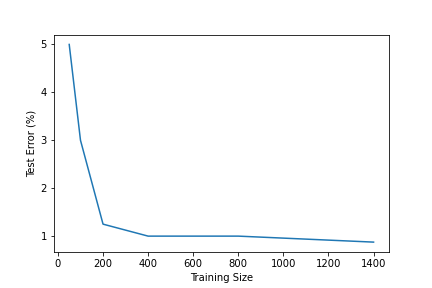
\includegraphics[width=4in,height=3.2in]{result.png} 
        \caption{Test error with the size of training set} 
    \end{figure}

    obviously, when the size of training set is equal to 1400, the error is the smallest, $0.87500\%$. Thus, size1400 gives the best set error.
    \pagebreak

    \textbf{Part c:} \\
    $\bullet$ Size of training set = 50: \\accuracy of naive bayes = $3.8750\%$ accuracy of SVM= $5.0000\%$ \\
    $\bullet$ Size of training set = 100: \\accuracy of naive bayes = $2.6250\%$ accuracy of SVM= $3.0000\%$ \\
    $\bullet$ Size of training set = 200: \\accuracy of naive bayes = $2.6250\%$ accuracy of SVM= $1.2500\%$ \\
    $\bullet$ Size of training set = 400: \\accuracy of naive bayes= $1.8750\%$ accuracy of SVM= $1.0000\%$ \\
    $\bullet$ Size of training set = 800: \\accuracy of naive bayes= $1.7500\%$ accuracy of SVM= $1.0000\%$ \\
    $\bullet$ Size of training set = 1400: \\accuracy of naive bayes= $1.6500\%$ accuracy of SVM= $0.8750\%$ \\
    Naive Bayes has better performance for smaller training sets and SVM has better performance for larger training sets.
\end{homeworkProblem}
\end{document}